%%%%%%%%%%%%%%%%%%%%%%%%%%%%%%%%%%%%%%%%%
% Masters/Doctoral Thesis 
% LaTeX Template
% Version 2.5 (27/8/17)
%
% This template was downloaded from:
% http://www.LaTeXTemplates.com
%
% Version 2.x major modifications by:
% Vel (vel@latextemplates.com)
%
% This template is based on a template by:
% Steve Gunn (http://users.ecs.soton.ac.uk/srg/softwaretools/document/templates/)
% Sunil Patel (http://www.sunilpatel.co.uk/thesis-template/)
%
% Template license:
% CC BY-NC-SA 3.0 (http://creativecommons.org/licenses/by-nc-sa/3.0/)
%
%%%%%%%%%%%%%%%%%%%%%%%%%%%%%%%%%%%%%%%%%

%----------------------------------------------------------------------------------------
%	PACKAGES AND OTHER DOCUMENT CONFIGURATIONS
%----------------------------------------------------------------------------------------

\documentclass[
12pt, % The default document font size, options: 10pt, 11pt, 12pt
oneside, % Two side (alternating margins) for binding by default, uncomment to switch to one side
english, % ngerman for German
onehalfspacing, % Single line spacing, alternatives: onehalfspacing or doublespacing
%draft, % Uncomment to enable draft mode (no pictures, no links, overfull hboxes indicated)
%nolistspacing, % If the document is onehalfspacing or doublespacing, uncomment this to set spacing in lists to single
liststotoc, % Uncomment to add the list of figures/tables/etc to the table of contents
%toctotoc, % Uncomment to add the main table of contents to the table of contents
JumpToContents, % Uncomment to add Jump to Contents href
parskip, % Uncomment to add space between paragraphs
%nohyperref, % Uncomment to not load the hyperref package
headsepline, % Uncomment to get a line under the header
%chapterinoneline, % Uncomment to place the chapter title next to the number on one line
%consistentlayout, % Uncomment to change the layout of the declaration, abstract and acknowledgements pages to match the default layout
]{MastersDoctoralThesis} % The class file specifying the document structure

\usepackage[utf8]{inputenc} % Required for inputting international characters
\usepackage[T1]{fontenc} % Output font encoding for international characters

\usepackage{mathpazo} % Use the Palatino font by default

%\usepackage[backend=bibtex,style=authoryear,natbib=true]{biblatex} % Use the bibtex backend with the authoryear citation style (which resembles APA)
\usepackage[backend=bibtex,style=iso-numeric,natbib=true]{biblatex}%verbose-trad2
\addbibresource{biblio.bib} % The filename of the bibliography

\usepackage[autostyle=true]{csquotes} % Required to generate language-dependent quotes in the bibliography

%----------------------------------------------------------------------------------------
%	Sorted Lists / reference to ToC SETTINGS 
%----------------------------------------------------------------------------------------
%\usepackage{verbatim}
\makeatletter\let\expandableinput\@@input\makeatother % needed for \expandableinput

\let\oldtableofcontents\tableofcontents
\renewcommand{\tableofcontents}{%
  \cleardoublepage
  \phantomsection% Place hyperlink marker
  \label{ToC-first-page}% Set \label for hyperlink
  \oldtableofcontents %t67
}

\usepackage[nobottomtitles*]{titlesec} % To avoid having a section title at the end of a page
%\usepackage[table]{xcolor} % To add alternating colors to rows in tables. Already in use.
\definecolor{light-gray}{gray}{0.96}

\newcommand{\specialcell}[2][t]{%
  \begin{tabular}[#1]{p{12.5cm}}#2\end{tabular}}
  
% \usepackage[acronym]{glossaries} % this adds acronyms to latex
% \makenoidxglossaries
% \newacronym{gmaw}{GMAW}{Gas Metal Arc Welding}
\newacronym{roi}{ROI}{Region of Interest} 
\newacronym{iqr}{IQR}{Interquartile Range} 
\newacronym{iqm}{IQM}{Inter Quartile Mean} 
\newacronym{std}{STD}{Standard Deviation} 
\newacronym{rfr}{RFR}{Random Forest Regressor}
    
%\usepackage{incgraph,tikz}
\usepackage{amsmath}
\usepackage{array}          % i dont remember
\usepackage{listings}       % add code snippets to pdf
\usepackage{varioref}       % adds page numbers to references. use \vref
\usepackage{hyperref}       % has to be loaded before cleveref
\usepackage[nameinlink]{cleveref}       % use \cref instead of \ref
\usepackage{float}          % use [float,floatplacement=H] to avoid page breaks in listings
\usepackage{placeins}       % provides command \FloatBarrier
\usepackage{wrapfig}
\usepackage{graphicx}
\usepackage{caption}
\usepackage{subcaption}
%\usepackage{multicol}
% \usepackage[british]{babel}
\usepackage[export]{adjustbox}

\usepackage{array}
\newenvironment{conditions}[1][Where:]
  {#1 \begin{tabular}[t]{>{$}l<{$} @{${}={}$} l}}
  {\end{tabular}\\[\belowdisplayskip]}


\usepackage{titlesec} % esto es para que los parrafos se comporten como secciones
\titleformat{\paragraph}
{\normalfont\normalsize\bfseries}{\theparagraph}{1em}{}
\titlespacing*{\paragraph}
{0pt}{3.25ex plus 1ex minus .2ex}{1.5ex plus .2ex}
\usepackage{makecell} %esto es para tener linebreaks dentro de table cells


\definecolor{codegreen}{rgb}{0,0.6,0}
\definecolor{codegray}{rgb}{0.5,0.5,0.5}
\definecolor{codepurple}{rgb}{0.58,0,0.82}
\definecolor{backcolour}{rgb}{0.95,0.95,0.92}
%\doublespacing

\usepackage{tikz}
\usetikzlibrary{arrows,shapes,positioning,shadows,trees}
\tikzset{
  basic/.style  = {draw, text width=2cm, drop shadow, font=\sffamily, rectangle},
  root/.style   = {basic, rounded corners=2pt, thin, align=center, fill=green!30},
  level 2/.style = {basic, rounded corners=6pt, thin,align=center, fill=green!60, text width=8em},
  level 3/.style = {basic, thin, align=left, fill=pink!60, text width=7em}
}

\lstdefinestyle{mystyle}{
    backgroundcolor=\color{backcolour},   
    commentstyle=\color{codegreen},
    keywordstyle=\color{blue},
    numberstyle=\tiny\color{codegray},
    stringstyle=\color{codepurple},
    basicstyle=\ttfamily\footnotesize,
    breakatwhitespace=false,         
    breaklines=true,                 
    captionpos=b,                    
    keepspaces=true,                 
    numbers=left,                    
    numbersep=5pt,                  
    showspaces=false,                
    showstringspaces=false,
    showtabs=false,                  
    tabsize=2,
    emph={GetVar, Wait, If, Message, Wait_Con, Calc, Endif, While, Wend},
    emphstyle={\color{magenta}\bfseries}
}
\lstset{style=mystyle}



% \makeatletter
% \newcommand*{\NoBreakPar}{\vspace{\baselineskip}\par\nobreak\@afterheading}
% \makeatother

%----------------------------------------------------------------------------------------
%	MARGIN SETTINGS
%----------------------------------------------------------------------------------------

\geometry{
	paper=a4paper, % Change to letterpaper for US letter
	inner=3.5cm, % Inner margin
	outer=1.5cm, % Outer margin
	bindingoffset=.5cm, % Binding offset
	top=3cm, % Top margin
	bottom=2.5cm, % Bottom margin
	%showframe, % Uncomment to show how the type block is set on the page
}

%----------------------------------------------------------------------------------------
%	THESIS INFORMATION / MY VARIABLES
%----------------------------------------------------------------------------------------
\subject{Special Aspects of Mobile Autonomous Systems} % \subjectname
\thesistitle{Autonomous Desk Organizer}    % \ttitle
\examiner{Prof. Dr.-Ing. Chunrong \textsc{Yuan}} % \examname

\university{\href{http://www.th-koeln.de}{Technische Hochschule Köln}}                    % title page and abstract \univname
\faculty{\href{}{F07 - Fakultät für Informations-, Medien- und Elektrotechnik}}   % title page and abstract \facname
\addresses{Köln} % \addressname

\author{Lu \textsc{Knoblich}, Christian \textsc{Schmitz}}
% \authora{Lu \textsc{Knoblich}} % title page/ abstract \authorname
% \authorb{Christian \textsc{Schmitz}} % title page/ abstract \authorname
\matrikelnra{373292}
\matrikelnrb{373292}

\timeperiod{February 15th, 2023}

\supervisor{SUPA} % \supname
\supervisorb{SUPB} % \supnameb

\keywords{} % \keywordnames
\semester{9}

% \department{\href{https://www.hs-kempten.de/hochschule/fakultaeten/elektrotechnik.html}{Mechatronic}}   % title page and abstract \deptname
% \group{\href{http://www.thyssenkrupp.de}{Thyssenkrupp}}                                        % research group's name, used in title page \groupname

\company{\href{}{COMPANY}}
\study{\textsc{STUDY}}

\headtitle{\ttitle}

%----------------------------------------------------------------------------------------
%   END OF MY VARIABLES
%----------------------------------------------------------------------------------------

\AtBeginDocument{
\hypersetup{pdftitle=\ttitle} % Set the PDF's title to your title
% \hypersetup{pdfauthor=\authornamea, \authornameb} % Set the PDF's author to your name
\hypersetup{pdfauthor=\authorname} % Set the PDF's author to your name
\hypersetup{pdfkeywords=\keywordnames} % Set the PDF's keywords to your keywords

}

\setlength\bibitemsep{0.5\baselineskip}
\begin{document}
\frontmatter % Use roman page numbering style (i, ii, iii, iv...) for the pre-content pages



\pagestyle{plain} % Default to the plain heading style until the thesis style is called for the body content
\rowcolors{1}{white}{light-gray}

%----------------------------------------------------------------------------------------
%	TITLE PAGE
%----------------------------------------------------------------------------------------



\begin{titlepage}
    % \begin{figure}[p]
    
    % \vspace*{-5cm}
    % \makebox[\linewidth]{
    %     \includegraphics[width=1.5\linewidth]{Chapters/Deckblatt}
    % }
    % \end{figure}
    
\iftrue
\begin{center}

\iffalse
    \begin{flushleft}
    \emph{Authors} \\
    \authorname
    % {\authornamea - \pmatrikelnra \\
    % \authornameb - \pmatrikelnrb}
    \end{flushleft}
    \begin{flushright} \large
    \emph{Matriculation Number} \\
    {\pmatrikelnra}
    {\pmatrikelnrb}
    \end{flushright}
\fi


\includegraphics[scale=0.15]{Figures/logo-thk.jpg}\\



% \vspace*{.06\textheight}
% {\scshape\LARGE \univname\par}\vspace{0.8cm} % University name
\textsc{\Large Project Report}\\[0.4cm] % Thesis type % Bachelor Thesis
Subject: \subjectname

\HRule \\[0.2cm] % Horizontal line
{\huge \bfseries \ttitle\par}\vspace{0.3cm}% at \compname \vspace{0.4cm} % Thesis title

% \authornamea, \authornameb \\
\authorname \\
\HRule \\[0.8cm] % Horizontal line



\begin{tabular}{r l}
\hiderowcolors
     \vspace{0.2cm}
     Prüfer: & \examname \\
     \vspace{0.2cm}
     Arbeit vorgelegt am: & \today  \\
     \vspace{0.2cm}
      % 
      % \vspace{0.2cm}
      Matrikel Nummer: & \pmatrikelnra,\pmatrikelnrb\\
      % \vspace{0.5cm}
    %  \vspace{0.2cm}
    %  Faculty: & \facname \\
    %  \vspace{0.2cm}
    %  Matriculation Number: & \pmatrikelnr \\
    %  \vspace{0.2cm}
    %  Place: & \addressname \\
\end{tabular}
\\[1.9cm]
 
\vfill
\end{center}
\fi
\end{titlepage}



\cleardoublepage %Double Space needed for first pages to be printed one-sided only. 
%\clearpage

%----------------------------------------------------------------------------------------
%	QUOTATION PAGE
%----------------------------------------------------------------------------------------

%\vspace*{0.2\textheight}

%\noindent\enquote{\itshape\textcolor{red}{ Thanks to my solid academic training, today I can write hundreds of words on virtually any topic without possessing a shred of information, which is how I got a good job in journalism.}}\bigbreak

%\hfill Dave Barry

%----------------------------------------------------------------------------------------
%	ABSTRACT PAGE
%----------------------------------------------------------------------------------------

\begin{abstract}
    \addchaptertocentry{\abstractname} % Add the abstract to the table of contents

    
    The workplace of the future is characterized by a high degree of automation, which is also reflected in the field of logistics. The aim of this project is to develop a robot that autonomously identifies, collects and organizes objects with the premise of having to organize a desk in such a way that the implementation is able to be easily adapted to other applications. The implementation of this project was done using the open source webots robotics simulation environment from cyberbotics.

    The robot is linked to a camera with a view of the desk surface and the objects on it, and a gripper that allows the objects to be grabbed. The robot is able to detect objects and their position with the use of a neural net trained on images of the objects available and the use of the openCV python module for subsequent image processing. With a defined sequence of movements, the robot is able to pick up the individual objects and place them in their corresponding location.

    Solution theory, implementations and documentation of the developed system are presented within this paper.

    
\end{abstract}



\tableofcontents % Prints the main table of contents

%----------------------------------------------------------------------------------------
%	THESIS CONTENT - CHAPTERS
%----------------------------------------------------------------------------------------

\mainmatter % Begin numeric (1,2,3...) page numbering
\pagestyle{thesis} % Return the page headers back to the "thesis" style

\chapter{Introduction} % 
\label{CH1} % \ref{CHX}
The purpose of this project is to address the problem of an cluttered work space.
The solution we developed is a robotic arm that is designed to clean up and organize the work area. 
In this report we will document and discuss the development process of the project. 

The report is comprised of three sections. The first part provides a general introduction to the Project, where the project idea as well as technology used will be addressed. The main section of this report is divided into two chapters: "Solution theory" and "Implementation".
The "Solution Theory" chapter addresses the problems that needed to be solved in order to realize the project and the corresponding theoretical solutions for these problems. 
The "Implementation" chapter provides detailed explanations of how the solutions were actually implemented and draws a comparison between the theoretical solution and the actual implementation. Finally, the last part of the report focuses on the project results and provides a conclusion, evaluating whether we have achieved our project goals and discussing further improvements for the project as well as learning outcomes. 

\section{Project Description}

The objective of the project is to create a robotic system capable of tidying and arranging a workspace. The design incorporates a camera that identifies objects within the area, which the robotic arm then grasps and relocates to a designated spot.

\begin{itemize}
    \item prove of concept for varios real world application
    \item Solution transferable to other use cases
\end{itemize}


In the initial phases of the project, the decision was made to utilize a simulation rather than a physical robot. This choice was made due to the ease of testing and development in a simulated environment. The Webots simulation platform was selected for its compatibility with the project, as it is an open-source simulation platform utilized for research and education purposes. The platform is based on the ODE physics engine and the OpenGl graphics library, and offers a broad array of sensors and actuators that can be utilized to develop a robot. Furthermore, Webots integrates various existing robot-devices so that the developed controllers can be used in the real world applications. We chose to use the Irb4600 robot, which is a six-axis industrial robot that is widely used in industry. Additionally the Webots API is provided in various programming languages, including C++, Python, Java, and Matlab. Due to the machine learning and computer vision components of the project, we decided to use Python to implement the developed solution, as it is widely supported in computer vision and machine learning applications. Git was used to manage the project and to facilitate collaboration between the team members.


\begin{figure}[!htbp]
    \centering
    \adjincludegraphics[width=0.7\textwidth]{Figures/project2.png}
    \caption{Figure 1: Project setup in Webots }
    %\label{fig:figure}
\end{figure}

Figure one shows the project setup in Webots. A camera is used to detect objects in the workspace. The robot-arm is equipped with a gripper that can be utilized to grasp objects. The robot and its devices are controlled by a controller that is responsible for detecting objects, determining the robot's movement, and controlling the gripper. The entire system is self contained and doesn't require human interaction, other devices or an active web connection.

The system was developed by a team of two students and divided into three main components: object detection, coordinate transformation, and robotic arm control. 


% !TEX root = ../main.tex

\chapter{Solution Theory} % Main chapter title
\label{theory} % \ref{theory}


This chapter addresses the solution concepts for the problems that needed to be solved in order to realize the project and is structured according to the previously mentioned main components of the project: object detection, coordinate transformation, and robotic arm control. 
 
\subsection{Object detection}
The first component of the project is the object detection. Its purpose is to detect objects in the workspace and determine their relative coordinates and size in the image as well as their orientation in relation to the table. 

To simplify these problems, we decided to use a top-down view of the workspace. This means that the camera is positioned above the workspace, so that a linear correlation between the image and the table coordinates emerges. At the early stages of project development the training of a custom object detection model was not intended and it was planned to utilize an existing model. The YOLOv3 model, a convolutional neural network that is trained to detect objects in images, was selected due to its wide array of object classes and its high performance.

To detect the orientation of an object relative to the table, we decided to use OpenCV, a python library used in computer vision applications which provides a broad array of functions for image processing. The main idea was to determine the contours of the object by converting the image into the HSV color space and applying different filter. The contours are then used to calculate the main orientation of the object, using principle component analysis. 

\subsection{Coordinates transformation}

Once the objects are detected, the next step is to determine their coordinates in the simulation. 

\begin{itemize}
    \item TODO: first / theoretical approach to solve problem(s)
\end{itemize}
Once knowing the coordinates of the detected object in the image, 
the next step is to transform the objects position vector from the image's coordinate system to the world's coordinate system. This type of transformation is best achieved with the use of a transformation matrix.

% <!-- the next step is to determine the coordinates of the object in the simulation environment so that its position relative to the robot arm can be used. -->

\subsubsection{Transformation Matrix}

Assuming a current coordinate system $\mathbf{A}$ and a target coordinate system $\mathbf{B}$, the transformation matrix $\mathbf{T}$ can be used to transform a vector $\vec{v}$ from $\mathbf{A}$ to $\mathbf{B}$.
A transformation matrix can be represented as a matrix frame, built from a combination of a rotation matrix, a translation vector, a scaling vector and a perspective projection matrix.

$$
\mathbf{T} = \left[
\begin{array}{ccc|c}
\ast&\ast       &\ast&\ast\\
\ast&\mathbf{R} &\ast&\vec{t}  \\
\ast&\ast       &\ast&\ast\\
\hline
\ast&\mathbf{P} &\ast&\mathbf{S}
\end{array}
\right]
$$
where:  
* $\mathbf{R}$ is the rotation matrix with the dimensions $3\times 3$.  
* $\vec{t}$ is the translation vector with the dimensions $3\times 1$.  
* $\mathbf{P}$ is the perspective projection matrix with the dimensions $1\times 3$.  
* $\mathbf{S}$ is the scale factor with the dimensions $1\times 1$ (for uniform or isotropic scaling).

The rotation matrix for a rotation around any given axis given by the unit vector $\mathbf{\vec{u}(x,y,z)}$ by an angle $\theta$ is given by the following formula:

$$
\mathbf{R} =
\begin{bmatrix}
u_x^2(1-\cos\theta) + \cos\theta & u_xu_y(1-\cos\theta) - u_z\sin\theta & u_xu_z(1-\cos\theta) + u_y\sin\theta \\
u_xu_y(1-\cos\theta) + u_z\sin\theta & u_y^2(1-\cos\theta) + \cos\theta & u_yu_z(1-\cos\theta) - u_x\sin\theta \\
u_xu_z(1-\cos\theta) - u_y\sin\theta & u_yu_z(1-\cos\theta) + u_x\sin\theta & u_z^2(1-\cos\theta) + \cos\theta \\
\end{bmatrix}
$$

If the rotation is performed around the z axis, the rotation matrix can be simplified to the following form:
$$
\mathbf{R} =
\begin{bmatrix}
\cos\theta & -\sin\theta & 0 \\
\sin\theta & \cos\theta & 0 \\
0 & 0 & 1 \\
\end{bmatrix}
$$


The translation vector is the position of the origin from current coordinate system $O_{current}$ 
relative to the target coordinate system $O_{target}$, i.e. the distance between both origins given as a three dimensional vector. 

$$
\vec{t} =
\begin{bmatrix}
x\\
y\\
z\\
\end{bmatrix}=
O_{current}-O_{target}
$$

The perspective projection matrix is not used in this project due to the camera orientation being perpendicular to the surface of intereset, but is included for completeness.

The scaling factor as given in the frame above can only be used for isotropic scaling, i.e. scaling in all three dimensions by the same factor. Since we are mainly interested in scaling in the x and y directions by different amounts, a single scaling factor can not be used by itself and needs to be expanded to a scaling matrix $\mathbf{S}$ with the following form:

$$
\mathbf{S}=
\begin{bmatrix}
S_x & 0 & 0   & 0\\
0 & S_y & 0   & 0\\
0 & 0   & S_z & 0\\
0 & 0   & 0   & 1
\end{bmatrix}
$$


where $S_x$, $S_y$ and $S_z$ are the scaling factors in the x, y and z directions respectively.

With the rotation and translation matrices a primary Transformation matrix $\mathbf{T_{0}}$ is built with the previously described frame using the unit 1 as a scaling factor and a null matrix as the perspective matrix. 
This is then multiplied with the scaling matrix $\mathbf{S}$ to obtain the complete transformation matrix $\mathbf{T}$ as follows. 

$$\mathbf{T} =  \mathbf{S} \bullet  \mathbf{T_{0}}$$

% <!-- 
% \textcolor{red}{ The following is not complete, needs to be reworked and checked } % end red

% This is done by dividing the dimensions of the table in the simulation by the dimensions of the table in the image. Knowing this, it is possible to generate a transformation matrix

% The first step is to determine the dimensions of the table in order to calculate the scale factor between the image and the simulation. Knowing the scale factor, it is necessary to determine the position and orientation of the table, in order to complete the transformation matrix that needs to be use to calculate the coordinates of the object in the simulation.

% A transformation matrix is a 4x4 matrix that is used to transform a vector from one coordinate system to another. The transformation matrix is calculated by multiplying the translation matrix, the rotation matrix, and the scale matrix. The translation matrix is used to translate the vector from the origin of the coordinate system to the desired position. The rotation matrix is used to rotate the vector around the origin of the coordinate system. The scale matrix is used to scale the vector to the desired size.



% In order to tranform the coordinates from the unit \(pixels\) to the unit \(meters\), the scale matrix is calculated as follows:

% $$
% \begin{bmatrix}
%  width & 0 & 0 & 0 \\
%  0 & height & 0 & 0 \\
%  0 & 0 & depth & 0 \\
%  0 & 0 & 0 & 1 \\
% \end{bmatrix}
% $$

% where \(width\), \(height\), and \(depth\) are the dimensions of the table in the simulation. -->

\subsection{Robot controller}

The robot controller is the main program where the behaviour of the robot is defined. It is responsible for the different actions that take place in the simulation. By marking the crobot as a supervisor in webots, it can access and modify the properties of other elements in the scene and the environment. 

The main tasks of the robot controller are the following:

\begin{itemize}
    \item Initialization of the different modules and devices
    \item calling of the image processing and object detection modules
    \item performing the required movements of the robotic arm
    \item controlling the movement of the gripper and its fingers
    \item coordinating the actions of the different modules
\end{itemize}

% <!-- 
% It manages and accesses the robot's motors and sensors, and by using the supervisor class from the webots API, it can also have access to the other devices and elements in the simulation. This class allows it to modify the simulation environment and the nodes that are present in the scene, It also provides the capability of accessing and modifying the properties of other elements in the simulation, as well as controlling how the simulation is run.

%  that controlls the robotic arm and accesses the different modules and devices in the simulation. The webots environment provides a supervisor class which provides the capability of accessing and modifyng the properties of other elements in the simulation, as well as controlling how the simulation is run. -->


% <!-- is responsible for the different actions that take place in the simulation. It manages and accesses the robot's motors and sensors of the actions and the access to the other devices in the simulation. It 

% Additionally, a robot-controller needs to be developed to control the robotic arm and the gripper.

% \begin{itemize}
%     \item TODO: first / theoretical approach to solve problem(s)
% \end{itemize}  
% These components will then be integrated into a single routine to detect objects, maneuver the robotic arm to the objects, and relocate the objects to a specified location. -->

\subsubsection{Robot Kinematics}


The Robot chosen for this task consists of a robotic arm with a gripper attached to the end of the arm. The robot by itself can be represented as a kinematic chain with 6 joints, resulting in 6 degrees of freedom.
In order to move the robot, the target angle of each individual joint in the kinematic chain needs to be set. Nevertheless, the position of the objects and target locations for the robot's movement are defined in a three dimensional coordinate system, so a transformation between the joint angles and the position of the end effector (last chain element) in space needs to be achieved in order to control its movements.

Calculating the position of the gripper (the end effector) from the known position of the individual motor can be achieved using a process called forward kinematics, which combines multiple applications of trigonometric formulas.

Nonetheless, the reverse operation, which aims to calculate the required position of the joints in the kinematic chain for a given position of the end effector presents a more challenging problem. 
This process called inverse kinematics (IK), for which different methods can be used. These methods can be divided into two categories: analytical and numerical.

The analytical methods are based on the use of trigonometric formulas, which can be used to calculate the required position values for the motors. However, these methods are limited to a specific number of degrees of freedom, and can only be used for a limited number of cases.

The numerical methods are based on the use of iterative algorithms, which can be used to calculate the required position values for the motors. However, while these methods are not limited to a specific number of degrees of freedom, they can be computationally expensive and are non-deterministic procedures, meaning there can be more than one solution for a given point. Likewise, the time required to find a solution is also non-deterministic, which poses a problem when critical computations need to be performed in real time.

\textcolor{red}{Insert image showing forward and inverse kinematics from Folien} % end red


\subsubsection{Gripper Actuation}

The gripper consists of three individual fingers, each of them having three joints. The closing action of the finger is achieved by rotating the first joint of each finger until the desired object is grabed or the maximum joint rotation is reached. This alone creates a claw like grip, since all finger sections rotate with the first joint relative to the global coordinates. While useful in some cases, its contact area with the object being grabbed is significantly reduced.

A different approach that aims to improve the contact area of the gripper, is possible rotate the last joint of each finger in the opposite direction by the same amount as the first one, compensating the rotation on the fingertips and creating a more stable grip.

The following figure shows the gripper in the open and closed position using the a claw and a pinch grip respectively.

\textcolor{red}{insert figure of gripper open, closed claw and closed flat} % end red


\subsubsection{Movement coordination}

The main loop of actions that need to be taken to complete the task of organizing the desk can be defined as seen in figure ASD. 

The process starts by moving the robot to a HOME position where it wont interfere with the camera's view of the desk. A picture is taken and any objects present are detected. If objects were detected, the robot iterates through the found objects, picking them up and placing them on the a second table on their corresponding position, until all the detected objects have been moved. The robot then moves back to the HOME position. If no object is detected, no movement of the robot takes place. This process is repeated until the user decides to stop the simulation.

\begin{lstlisting}[]%language=plantuml
@startuml
:**Simulation Start**;
repeat :Move Robot to HOME Position;
    repeat :Take Picture;
        :Perform Object Detection;
    repeat while (objects found?) is (no) not (yes)

    repeat :Coordinate Transformation;
        :Move object;
        :Remove from found objects;
    repeat while (more objects?) is (yes)
repeat while (Keep Watching?) is (yes)
:stop;
@enduml
\end{lstlisting}

\textcolor{orange}{
. moves to pick up the object and places  
Being able to detect the objects position and orientation, and moving 
With the information regarding the objects' position and orientation in the simulation, the following step is to control the robots movement to produce the desired behavior. The robot controller is implemented in Python and uses the Webots API to control the robot. The robot controller is responsible for the following tasks:
}

\textcolor{orange}{
Initialization of the robot instance and the devices attached to it: 
* camera
* gripper
* internal variables
* Motor sensors
* Motor actuators
}

\textcolor{orange}{
Coordination of the robot's movement.
Coornidation of the different steps required for the organization process.
* Reding the camera's image and forwarding the data to the object detection module.
* Reading the object detection module's output and forwarding the data to the coordinate transformation module.
* Reading the coordinate transformation module's output and forwarding the data to the robotic arm control module.
* Perform the movement as required for the detected objects positions
} %end orange


% !TEX root = ../main.tex
\chapter{Implementation} % Main chapter title

\label{implementation} % \ref{CHX}


In this chapter we will describe the implementation of the solutions proposed in the previous chapter. Additionally, there will be a comparison between the theoretical solution and the actual implementation as well as a discussion of the difficulties that were encountered during the development process. The chapter is structured according to the previously mentioned main modules of the project: object detection, coordinate transformation, and robotic arm control.
\section{Object detection}

\subsection{First approach}
The first approach to solve the problem of object detection was to use the YOLOv3 model. The model was trained on the COCO dataset, which contains 80 different object classes. During the early stages of development we setup a test scenario in Webots, where we placed various objects in the workspace and used the YOLOv3 model to detect the objects. 

\Vref{fig:object_detection_results} shows the results of the object detection using the YOLOv3 model. The following objects on the workspace are included in the COCO dataset and should therefore be detectable by the model: computer mouse, apple, beer can and orange. The camera perspective in this test scenario was similar to the perspective in the final project setup.  

\begin{figure}[!h]
    \centering
    \adjincludegraphics[width=\textwidth]{Figures/cvResultExistingModel.jpg}
    \caption{Object detection results YOLOv3 model }
    \label{fig:object_detection_results}
\end{figure}


The model was able to detect the beer can with an accuracy of 94 percent. However, the orange only had a likelihood of 71 percent whereas the apple and the computer mouse were not detected at all. Although the model was able to identify the beer can the overall performance was not satisfactory and another solution was needed.

\subsection{Second approach}

The second approach to solve the problem of object detection was to train a custom model. In the project plan, it was not initially planned to train an own model. However, to streamline the process, the decision was made to utilize the ImageAI library, a python library that offers a convenient framework for training and utilizing object detection models. \autocite{ImageAI}

In order to reduce the effort needed to train the model, we decided to use transfer learning, which is a machine learning method where a model, trained on a large dataset, is used as a starting point for a new model. The new model is then trained, containing the pre-trained weights of the origin model. \autocite{mlearning} We chose to use the pre-trained YOLOv3 model, mentioned above, as the basis for transfer learning. 

\subsection{Training data }

The first step to train a custom model is to gather and arrange the training data in the YOLO annotation format. In this format the data is divided into two main directories: "train" and "validation". Each of these directories contains two sub-directories: "images" and "annotations". It's recommended to use 80\% of the data for training and 20\% for validation. The data consists of both images of objects we want to detect and accompanying annotation files. Each image is linked with a corresponding annotation file that shares the same name as the image file and provides information about the objects in the image. The general structure of the object annotation is shown below. 

\begin{lstlisting}[language=prolog]
<object-class><x-pos><y-pos><width><height>
\end{lstlisting}

The file contains one line for each object in the image. The object class is an integer that represents the type of the object. The value corresponds to a list of objects in another file named "classes.txt" inside the "annotation" directory and is encoded by the index of the object in the list. The x-pos, y-pos, width, and height are the information for the bounding box of the object in the image. The values are normalized to the range [0, 1] and are relative to the width and height of the image.

\subsubsection{Automatization}

Instead of creating and labeling the images manually we decided to automate the process. The plan was to utilize the object detection feature integrated in Webots to automatically generate the image and annotation files within their respective directories. We only utilized this detection method to create training data, as the detection is not based on image recognition but hard coded within Webots. 

Two configurations were set up to generate training data. The first setup produces data with a top-down camera view and multiple objects arranged on the table. The second setup generates images with individual objects positioned on the table at different orientations and rotated camera at four distinct viewpoints.

\subsubsection{Configuration 1: Top down}

The initial step in realizing the top-down configuration involved the definition of a function for capturing camera images and generating the corresponding annotation files. This function utilizes a reference of the camera object to obtain the objects currently detected, determine the values needed for annotation and store the images in their designated directories. The following code segment demonstrates a shortened version of the implementation of this function.

\begin{lstlisting}[language=python]
def createTrainingFiles(camera,type = "train"):
   ... # initialize variables and generate pathes
   while True: # get current fileName
      filename = f"image_{fileNamePostfix}.txt"
      filepath = os.path.join(annotationPath, filename)
      if not os.path.isfile(filepath): 
          break # if file does not exist, use this name
      fileNamePostfix += 1
  fileName = f"image_{fileNamePostfix}"
  for obj in recognizedObjectes:
      id = obj.getId()
      name = obj.getModel()
      if name not in categories:
          continue
      position = list(obj.getPosition())
      positionOnImage = list(obj.getPositionOnImage())
      orientation = list(obj.getOrientation())
      size = list(obj.getSize())
      sizeOnImage = list(obj.getSizeOnImage())
      relativeSize = [sizeOnImage[0]/imageWidth, sizeOnImage[1]/imageHeight]
      relativePosition = [positionOnImage[0]/imageWidth, positionOnImage[1]/imageHeight]
      yoloData.append(f"{categories.index(name)} {relativePosition[0]} {relativePosition[1]} {relativeSize[0]} {relativeSize[1]}\n")
      jsonData.append({
          "id": id,
          ... # adding the remaining properties to json data
      })
  camera.saveImage(imagePath+fileName+".jpg",100) # save image
  with open(jsonPath+fileName+".json", 'w') as file: # save json data
      json.dump(jsonData, file, indent=4)   
  with open(annotationPath+fileName+".txt", 'w') as file: # save yolo annotation
      file.writelines(yoloData)
\end{lstlisting}
The function accepts two parameters, a reference to the camera object, and a "type". The purpose of the "type" parameter is to specify whether the function should generate training or validation data. The function starts by initializing various variables and generating file paths for the image, annotation, and JSON data. In addition to the required training data, all available information about an object was saved in a JSON file so that it can be used later. The JSON file shares the same name as the image file and is stored in the directory \(raw\_data\). Lines 3-8 determine the current file name for the output files. The filename is generated by appending a postfix to the string \(image\). The postfix is generated by incrementing a counter until a file with the generated name does not exist. This ensures that the file name is unique and does not overwrite existing files.
At line 10 a loop iterates over the objects that the camera recognizes, and collects information about each object, including its model name, position and size. These values are converted into the required format, by determining the object's relative position and size. Subsequently, in lines 22 and 23, strings for the annotation and the JSON representation of the detected object are prepared so they can be appended to the corresponding lists for this image. Finally, the function saves the image, JSON data, and YOLO annotation data to their respective files using the file name generated earlier. The image is saved using the camera's "saveImage" function.

After a snapshot was taken the object's position and orientation on the table needed to be randomized. The function to realize the object randomization is shown below.

\begin{lstlisting}[language=python]
def moveTableNodes(supervisor,table):
   margin = 0.1
   bottomLeft = table.local2world([0,1,0])
   topRight = table.local2world([1,0,0])
   x_min = bottomLeft[0] + (topRight[0] - bottomLeft[0]) * margin
   x_max = topRight[0] - (topRight[0] - bottomLeft[0]) * margin
   y_min = bottomLeft[1] + (topRight[1] - bottomLeft[1]) * margin
   y_max = topRight[1] - (topRight[1] - bottomLeft[1]) * margin
  for cat in categories:
       obj = supervisor.getFromDef(cat)
       x = random.uniform(x_min, x_max)
       y = random.uniform(y_min, y_max)
       z = bottomLeft[2] # any z coordinate
       obj.getField('translation').setSFVec3f([x, y, z])
       xRotation = random.uniform(1, 360)
       yRotation = random.uniform(1, 360)
       zRotation = random.uniform(1, 360)
       angle = random.uniform(1, 360)
       obj.getField('rotation').setSFRotation([xRotation,yRotation,zRotation,angle])

\end{lstlisting}
The function accepts two parameters: a reference to the supervisor object and a reference to the table object. The method begins by determining the boundaries of the table using coordinate transformation. Intervals for the x and y coordinates are determined for the random positioning of objects on the table and then adjusted to leave a margin of 0.1 meters around it. At line 9 a loop iterates the objects on the table and generates a random position and orientation for each object using the previously calculates intervals.

Finally a loop needed to be developed to call the snapshot and object randomization functions a specified number of times with a certain delay between each iteration. A decorator was used to extend the function to be repeatedly called until a specified condition is met while advancing the simulation. The following code segment demonstrates the implementation of this loop. 

\begin{lstlisting}[language=python]
@looper
def randomPosSamplingLoop(self,sampleSize,type):
    if self.loopCount % 10 == 0:
        if self.loopCount % 20 == 0:
            TrainingsHelper.moveTableNodes(self.supervisor,self.mainTable)
        else:
            TrainingsHelper.makeSnapshot(self.camera,type)
            self.dataCount +=1
    self.loopCount += 1
    if self.dataCount>sampleSize:
        return -1
\end{lstlisting}
The function takes two arguments as input: the quantity of samples, and the type of data, to be generated. In operation, the function initiates the execution of the \(moveTableNodes\) function at regular intervals of 20 iterations, ensuring the repositioning and reorientation of the objects every 2 seconds. Additionally, the \(makeSnapshot\) function is called every 10 iterations to secure the capturing of snapshots at a rate of once per second. The function concludes its operation by returning a value of -1 when the predetermined number of samples has been generated.

The method must be invoked twice, once for the generation of training data and once for the generation of validation data. Upon the completion of this process, a dataset is produced that is ready for the training of a custom model. \Vref{fig:dataset_train_img} and \Vref{fig:dataset_train_ann} present a dataset sample, generated by with this configuration, containing the image and its accompanying annotation file.

\begin{figure}[!h]
    \centering
    \adjincludegraphics[width=\textwidth]{Figures/image_344.jpg}
    \caption{image\_344.jpg in image directory  }
    \label{fig:dataset_train_img}
\end{figure}

\begin{figure}[!h]
    \centering
    \adjincludegraphics[width=\textwidth]{Figures/image_344.txt.jpg}
    \caption{image\_344.txt in annotations directory  }
    \label{fig:dataset_train_ann}
\end{figure}

We generated 1200 images for training and 300 images for validation using this configuration. In order to enhance the performance of the model, an alternative image configuration was also developed.

\subsubsection{Configuration 2: Four-angled rotation}

The second configuration was designed to provide single object images at four distinct viewpoints, serving as training data. To achieve this, a function was created to relocate the camera to a designated viewpoint. This function accepts two inputs: a reference to the supervisor object and an index specifying the desired viewpoint. The supervisor is used to alter the camera perspective while index is utilized to determine the camera's position based on a list of coordinates. Furthermore, a function was implemented to facilitate the exchange of objects on the table. This function takes three inputs as arguments: a reference to the supervisor object, a reference to the table object, and an index indicating the desired object. Finally, a function was created to randomly modify the orientation of the current node-object, resulting in a diverse set of images taken from the same viewpoint. After the completion of these steps, a routine was implemented that integrates the various functions. The code segment below presents the implementation of this function. 

\begin{lstlisting}[language=python]
def single_objectImage_setup(supervisor,table,imagesPerViewpoint):
    global count, currentNode, lastViewPointPos
    amountViewpoints = 4
    if(count==0): # init viewpoint position for first run
        moveViewPoint(supervisor,lastViewPointPos)
        swapObj(currentNode,table,supervisor)
    # change viewpoint if given imagesPerViewpoint is met
    if((count % imagesPerViewpoint) == 0):
        lastViewPointPos = (lastViewPointPos+1)%4
        moveViewPoint(supervisor,lastViewPointPos)
    # change object if limit is met
    if((count % (imagesPerViewpoint*amountViewpoints))==0):
        currentNode = (currentNode+1) % len(categories)
        swapObj(currentNode,table,supervisor)
    spinTableNode(supervisor,table,currentNode)
    count += 1
\end{lstlisting}
The function is meant to be executed each time after an image has been created and prepares the next image to be captured. The number of image configurations provided by the function is determined by the value of "imagesPerViewpoint". A global variable is used to keep track of the number of function invocations. The first time this method is called, the viewpoint and the first object are initialized. The if statement at line 8 verifies whether the number of images taken from the current viewpoint has reached the predetermined limit. In the event that the limit has been met, the viewpoint is shifted to the next one in the designated list. At line 12, the an if statement determines whether the number of images captured from the current object has reached its limit. If this is the case, the object is swapped for the next one in the list. Finally, the function rotates the current object to a random orientation with each invocation. 

The training data can be generated using the same function as in the first configuration. The loop to call these functions during the simulation closely mirrors the looper-function used before. The code segment below demonstrates the implementation of the method. 

\begin{lstlisting}[language=python]	
@looper
def singleObjectImageLoop(self,imagesPerPerspective,type):
    if self.loopCount % 10 == 0:
        if self.loopCount % 20 == 0:
            TrainingsHelper.single_objectImage_setup(self.supervisor,self.mainTable,imagesPerPerspective)
        else:
            TrainingsHelper.makeSnapshot(self.dataCam,type)
            self.dataCount +=1
    self.loopCount += 1
    if self.dataCount>imagesPerPerspective*amountPerspectives*len(categories): 
        return -1
\end{lstlisting}

This loop operates similar to the first configuration, alternately executing the \(single\_object\_setup\) and \(makeSnapshot\) functions with a set time delay. The termination criteria for this loop has been revised to ensure that the number of iterations is equal to the product of the amount of images per perspective, the number of perspectives, and the number of objects. In this configuration, we generated 256 training images and 64 validation images per object, capturing diverse orientations of the object from 4 different viewpoints.

\subsection{Training }

A total of 1456 images were generated for training and 384 images for validation. The training was performed using the ImageAI library, which provides a pre-trained YOLOv3 model that was used as a starting point for transfer learning. The following code segments presents the implementation of the training function, using the ImageAI library. 

\begin{lstlisting}[language=python]
def startTraining():
    execution_path = os.path.dirname(__file__)
    data_dir_path = os.path.join(execution_path , "DataSet")
    model_path = os.path.join(execution_path , "Modelle/yolov3.pt")
    createClassFiles(categories) 
    trainer = DetectionModelTrainer()
    trainer.setModelTypeAsYOLOv3()
    trainer.setDataDirectory(data_directory=data_dir_path)
    trainer.setTrainConfig(object_names_array=categories, batch_size=32, num_experiments=100, train_from_pretrained_model=model_path)
    trainer.trainModel()
\end{lstlisting}
The function sets up the data directory, model path, and configuration for the training process. It also creates the class files for the categories to be detected and initiates the training process using the "trainModel" method. The "DetectionModelTrainer" class from the ImageAI library is used to set up and train the model, with parameters such as batch size, number of training experiments, and object categories specified. 

The batch size was set to 32, while the number of training iterations through the dataset was set to 100. The training process was performed on a desktop computer using a NVIDIA GeForce RTX 4080 graphics card, an AMD Ryzen 7 5800X3D processor and 32 GB of ram. The training process took approximately 8 hours to complete.


\subsection{Result }

The results of the training after the 100th iteration are presented below.

\begin{lstlisting}[language=python]
    recall: 0.748433 precision: 0.683522 mAP@0.5: 0.736085, mAP@0.5-0.95: 0.340358
\end{lstlisting}

The results of the evaluation revealed that the model achieved a recall value of 0.748433, precision value of 0.683522, mAP@0.5 value of 0.736085, and mAP@0.5-0.95 value of 0.340358. 

The recall value of 0.748433 indicates that the model correctly detected 74.84\% of all positive instances present in the test dataset. Precision measures the proportion of detected instances that were correctly identified as positive. The precision value of 0.683522 suggests that 68.35\% of the instances detected by the model were positive. The mAP (Mean Average Precision) metric is a measure of accuracy in object detection tasks. The mAP@0.5 value of 0.736085 indicates that, on average, the model achieved a precision of 73.60\% in detecting objects in the test dataset, with a threshold of 0.5 for Intersection over Union (IoU) between the ground-truth and predicted bounding boxes. The Intersection over Union is a metric used to evaluate the similarity between two bounding boxes and measures the ratio of the area of intersection between the two boxes to the area of their union. Similarly, the mAP@0.5-0.95 value of 0.340358 suggests an average precision of 34.03\% in detecting objects using a range of IoU thresholds from 0.5 to 0.95. 

The low mAP@0.5-0.95 score indicates that the model is more likely to detect multiple bounding boxes for the same object with a high probability. \Vref{fig:trained_model_results} shows the results of the object detection process using the custom model and demonstrates the problem. 

\begin{figure}[!h]
    \centering
    \adjincludegraphics[width=\textwidth]{Figures/snapshot-detected-nms0.5.jpg}
    \caption{Object detection results self trained model }
    \label{fig:trained_model_results}
\end{figure}

Multiple bounding boxes with high probabilities were created respectively for each object, leading to distorted results, which is a common problem in object detection tasks. One possible reason for this issue could be overfitting, where the model has been trained for an extended period and has memorized the training data. Another possible cause could be an insufficient training dataset, which lacks diversity in its data, as it only provides a limited number of image configurations, despite the dataset's scope being sufficient.

The problem can be addressed by using non-maximum suppression (NMS) to find the best fitting box based on a given threshold. The NMS algorithm is implemented in the ImageAI library and can be used by setting the \(nms\_threshold\) parameter in the corresponding function. The NMS threshold is used to determine when two bounding boxes should be considered duplicates and only one should be kept. If the overlap between two bounding boxes, measured by the IoU, is greater than or equal to the NMS threshold, then  the bounding boxes with the lower confidence score will be eliminated alternatively both bounding boxes will be kept, as they are considered to be separate detections. By setting the NMS threshold to a certain value, the algorithm can eliminate duplicates and produce a cleaner, more accurate output. 

The results of the object detection process using The NMS algorithm with a threshold of 0.05 are presented in \vref{fig:trained_model_results_2}.

\begin{figure}[!h]
    \centering
    \adjincludegraphics[width=\textwidth]{Figures/snapshot-detected.jpg}
    \caption{Object detection results self trained model }
    \label{fig:trained_model_results_2}
\end{figure}

The test results indicate that the model has a satisfactory level of performance for the intended application, as it was capable to correctly determine the position and class of each object on the table in multiple test cases. 

To use the model during simulation a class was implemented to handle the object detection process. The class contains a method to detect objects in a given image, returning a list of detections and their respective bounding boxes as well as the corresponding orientation.

\section{Orientation of the object}

To determine the angle of an object relative to the table, the cv2 library was utilized. The approach relies on Principle Component Analysis (PCA) to determine the primary orientation of the object's contours. The function used to prepare the image for the orientation analysis is presented below.

\begin{lstlisting}[language=python]
def getAngle(self, objectImage, name: str|None = None, savefig: bool|None = None) -> float:
        try:
            # (1) Image of object is cropped using the bounding box and passed as a parameter
            # (2) Convert the image to the HSV color space
            hsv_image = cv2.cvtColor(objectImage, cv2.COLOR_BGR2HSV)
            # (3) Apply Canny edge detection
            edges = cv2.Canny(hsv_image, 50, 150)
            # Init masks
            leftEdgeMask=np.full(np.shape(edges),0)
            rightEdgeMask=np.full(np.shape(edges),0)
            topEdgeMask=np.full(np.shape(edges),0)
            bottomEdgeMask=np.full(np.shape(edges),0)
            # Init Boundary
            leftEdge=[1000 for i in range(np.shape(edges)[0])]
            rightEdge=[0 for i in range(np.shape(edges)[0])]
            topEdge=[1000 for i in range(np.shape(edges)[1])]
            bottomEdge=[0 for i in range(np.shape(edges)[1])]
            # Position Boundary
            for y,x in pos:
                leftEdge[y] = min(leftEdge[y],x)
                rightEdge[y] = max(rightEdge[y],x)
                topEdge[x] = min(topEdge[x],y)
                bottomEdge[x] = max(bottomEdge[x],y)
            # Make Masks from Boundary
            for y,x in enumerate(leftEdge):
                leftEdgeMask[y,x:] = 255
            for y,x in enumerate(rightEdge):
                rightEdgeMask[y,:x] = 255
            for x,y in enumerate(topEdge):
                topEdgeMask[y:,x] = 255
            for x,y in enumerate(bottomEdge):
                bottomEdgeMask[:y,x] = 255
            # (4) Remove inner edges by applying a mask to the image
            combined_mask = (leftEdgeMask*rightEdgeMask*bottomEdgeMask*topEdgeMask/255**3)
            # (5) Applying gaussian blur to smoothen edges
            blur = cv2.GaussianBlur(combined_mask, (11,11), 0)
            # (6) Using canny algorithm again to detect contours
            cleanEdges = cv2.Canny(blur.astype('uint8'),50,150)
            # (7) Using PCA (Principal Component Analysis) to compute the main orientation of the object
            orientation, contourNangle = self.getOrientationPCA(cleanEdges,objectImage)
            return orientation
\end{lstlisting}

The first step is to crop an image of the object using the bounding box coordinates provided by the object detection class. The image is then converted to the HSV color space and edges are detected using the Canny algorithm from the OpenCV library. The next step is to remove the object's inner edges by applying a mask to the image. This mask is created by selecting all the pixels that do not have any edge pixels between itself and at least one of the image's borders.

The edges are then smoothed using a Gaussian blur and contours are detected using the Canny algorithm a second time. Finally, the main orientation of the object is computed using the function "getOrientationPCA", presented in the following code segment.

\begin{lstlisting}[language=python]
def getOrientationPCA(self, edges):
    pts = np.transpose(np.where(edges>1),[1,0]).astype(np.float64)
    # Perform PCA analysis
    mean = np.empty((0))
    mean, eigenvectors, eigenvalues = cv2.PCACompute2(pts, mean)
    angle = math.atan2(eigenvectors[0,1], eigenvectors[0,0]) # orientation in radians
    return angle
\end{lstlisting}
This approach to determining the orientation of an object is based on the assumption that the main orientation of an object can be determined by finding the eigenvector with the highest variance in the dataset of edge points. OpenCV's principal component analysis implementation is used to find the eigenvectors of the dataset. The angle to the x-axis of the eigenvector with the highest variance is then calculated and returned as the main orientation of the object. The implementation of the function is partially based on an implementation example. \autocite{orientation}

A graphical representation of these steps is shown in \vref{fig:orientation_steps}, which highlights the individual images of the object at different stages of the process. 

\begin{figure}[!h]
    \centering
    \adjincludegraphics[width=\textwidth]{Figures/hammerTime.jpg}
    \caption{Steps do determine the orientation of an object }
    \label{fig:orientation_steps}
\end{figure}

The annotations below the images correspond to the respective steps in the "getAngle" function and are referred to in the comments of the function.

The first image corresponds to the original cropped section containing the object of interest. The second image displays the result obtained by performing a conversion to the HSV color space. This was performed to improve the distinction of edges between areas with different hues. Applying the Canny algorithm to this produces the third image as a result. The fourth image shows the area obtained by selecting all the pixels not encased by the detected edges. Applying a gaussian blur to this results in smoother edges as can be seen in the fifth image. Performing a second pass of the Canny algorithm results in what can be seen in the sixth image. Lastly, the seventh image shows the original cropped section of the object with an overlay displaying the direction of the eigenvectors, which determines the rotation of the object in relation to the fixed coordinate system of the image.

\section{Coordinate transformation}
\label{imp_transformation}

With relative position of the objects within the image, this position vectors need to be transformed to the world coordinate system to be able to set the target position of the robot. 
This task was achieved by creating and combining two different transformation matrices. The general procedure was implemented as follows:


\begin{lstlisting}[language=python]
# Transformation Matrix from table corner in image to table center
# - Rotation and Translation Matrix
img2table_rot_trans = [[0, -1,  0, 0.5],
                      [-1,  0,  0, 0.5],
                      [ 0,  0, -1,   1],
                      [ 0,  0,  0,   1]]

# - Scaling Matrix
img2table_scale = [[Table.size[0],             0,             0,  0],
                   [            0, Table.size[1],             0,  0],
                   [            0,             0, Table.size[2],  0],
                   [            0,             0,             0,  1]]

# Transformation Matrix from image to table center
img2table = numpy.matmul(img2table_scale, img2table_rot_trans)

# Transformation Matrix from table center to world
table2world = numpy.array([[cos(Table.rotation[3]), -sin(Table.rotation[3]),  0,  Table.position[0]],
                           [sin(Table.rotation[3]),  cos(Table.rotation[3]),  0,  Table.position[1]],
                           [                     0,                       0,  1,  Table.position[2]],
                           [                     0,                       0,  0,                 1]])

# Transformation Matrix from image to world
TMatrix = numpy.matmul(table2world, img2table)
\end{lstlisting}

Since the origin of the table's coordinate system is in the center of the table and therefore the table's position and orientation reference its center point, a translation needs to be applied to the position vector in the image, whose coordinate system is located on the top left corner, while also rotating the coordinate axes to match the ones of the table's origin (\Vref{fig:table_coords}).

\begin{figure}
    \centering
    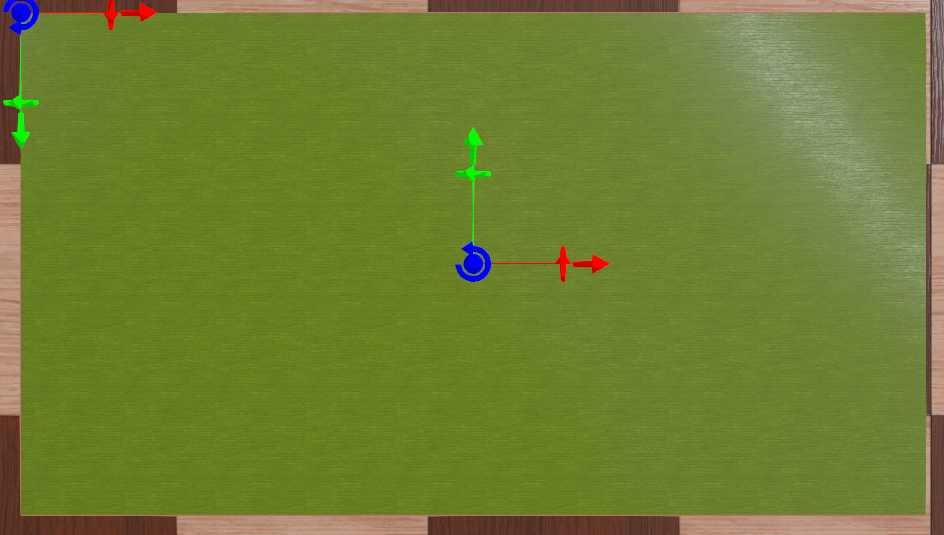
\includegraphics[width=\textwidth]{Figures/table_coords.png}
    \caption{Coordinate systems of the table and the image}
    \label{fig:table_coords}
\end{figure}

A second matrix is then used to scale the position vector to the dimensions of the table with the help of the Table's properties supplied by the webots API.

The rotation-translation matrix $\mathbf{M_{rt}}$ is then multiplied with the scaling matrix $\mathbf{M_s}$ to produce the transformation matrix $\mathbf{M_{img2table}}$ from the image coordinate system to the table coordinate system.

$$\mathbf{M_{img2table}} = \mathbf{M_s} \cdot \mathbf{M_{rt}}$$

A second transformation matrix is then responsible for transforming the position vector from the table coordinate system to the world coordinate system. For this implementation, a level table surface parallel to the XY plane is assumed, only allowing a rotation of the table in the Z axis. The rotation matrix is created from the rotation vector of the table, and the translation is taken from its position vector relative to the world origin, resulting in the transformation matrix $\mathbf{M_{table2world}}$.

These two transformation matrices are then multiplied with one another to produce a final transformation matrix $\mathbf{M_{img2world}}$ in order to directly transform the position vector from the image coordinate system to the world coordinate system.

$$\mathbf{M_{img2world}} = \mathbf{M_{table2world}} \cdot \mathbf{M_{img2table}}$$

In order to perform the actual transformation, the position vector needs to be augmented with a fourth value of 1, and is then multiplied with the transformation matrix to produce the final position vector in the world coordinate system.

$$\mathbf{v_{world}} = \mathbf{M_{img2world}} \cdot \mathbf{v_{img}}$$


\section{Robot arm}


\subsection{Robot Movement}

For the current implementation of the robot controller, some key decisions were made with the goal of preventing collisions with other objects in the scene during the robot's movement and increasing the predictability of the robot's behaviour:

\begin{itemize}
    \item objects are to be approached from above
    \item the gripper has to be pointing downwards while picking up or laying down an object, so as to provide a predictable hold of the object.
    \item the movement of the robot needs be deterministic, so as to avoid unexpected erratic movements
\end{itemize}

Taking these requirements into account, preliminary implementations to solve the inverse kinematics problem were made. The first of themused the full chain of the robot's joints and the python module "ikpy" to iteratively find the robot configuration required to reach a point in space.

The second implementation made use of the restrictions to the robots movement previously mentioned to utilize a reduced kinematic chain of only the joints that are relevant to the movement of the gripper.
Since the gripper is required be pointing down, the rotation of the fourth joint is restricted to the a value of zero, and therefore reduces the degrees of freedom of the kinematic chain by one. Likewise the fifth and sixth joints are constrained by a value defined only by the configuration of the first three joints, further reducing the degrees of freedom of the kinematic chain by two.

The following section describes the implementation of the second solution, which was chosen for the final implementation due to its deterministic nature and pretictable outcomes fullfilling the criteria previously mentioned. Furthermore, having a deterministic computation time results in an implementation that could be used with more reliability in other applications in which critical timing constraints are present.


\Vref{fig:simplified_kinematic} shows the robot's simplified kinematic chain with the resulting geometry used in the calculation of the required motor positions.


\begin{figure}[!h]
    \centering
    \adjincludegraphics[width=\textwidth]{Figures/simple_ik_geometry.png}
    \caption{Inverse Kinematic algorithm for the simplified kinematic chain.}
    \label{fig:simplified_kinematic}
\end{figure}


The position of the first motor $\omega_0$ can be calculated by removing the z component of the position vector $\vec{p_{xyz}}$, resulting in the vector $\vec{p_{xy}}$ and finding the angle $\omega_0$ produced between $\vec{p_{xy}}$ and the x axis $\vec{e_x}$ of the coordinate system with the following formula:

$$\omega_0=\arctan{\frac{y}{x}}$$

This procedure is represented geometrically on the left side of \vref{fig:simplified_kinematic}

The position of the second and third motors $\omega_1$ and $\omega_2$ can be represented on the plane produced by the the vector $\vec{p_{xy}}$ and the z axis $\vec{e_z}$ and calculating using the following formulas:

$$\omega_1=\frac{\pi}{2} - (\arctan{\frac{z}{h}} + \arccos{\frac{a^2-b^2+c^2}{2ac}})$$
$$\omega_2 = \frac{pi}{2} - \arccos{\frac{a^2+b^2-c^2}{2ab}} + r_{\omega_2}$$

\begin{conditions}
    a & length of the first link in the kinematic chain\\
    b & effective length of the second link in the kinematic chain\\
    c & distance between the origin of the coordinate system and the point of interest $\vec{p_{xyz}}$\\
    r_{\omega_2} & angle correction for $\omega_2$, required due to the second link's geometry.\\
\end{conditions}

% where:
% \begin{itemize}
%     \item $a$ is the length of the first link in the kinematic chain
%     \item $b$ is the effective length of the second link in the kinematic chain
%     \item $c$ is the distance between the origin of the coordinate system and the point of interest $\vec{p_{xyz}}$
%     \item $r_{\omega_2}$ is the angle correction for $\omega_2$, required due to the second link's geometry.
% \end{itemize}
Since the end effector is required to be pointing downwards, the angle $\omega_3$ corresponding to the fourth joint needs to be kept at 0.

$$\omega_3 = 0$$

The angle $\omega_4$ corresponding to the fifth joint is also required to be set such that the end effector is pointing downwards. This is achieved by rotating the joint to compensate the rotation of the angles $\omega_1$ and $\omega_2$ while also offsetting the rotation by 90 degrees to point downward instead of forward.

$$\omega_4 = \frac{\pi}{2} - (\omega_1 + \omega_2)$$

The rotation of the sixth joint $\omega_5$ corresponding to the rotation of the gripper is set to have a default value, such that the gripper's grabbing orientation is pointing parallel to the x-axis. This is done by setting its rotation $\omega_5$ to compensate the rotation $\omega_0$ of the first joint. Since the $z$ axis of first and sixth joint are pointing in opossite directions, these two rotations can take the exact same value. An angle $\theta$ with a default value of $0$ is added to the rotation of the sixth joint to allow for different orientations of the gripper.

$$\omega_5 = \omega_0 + \theta$$


The complete implementation was done as follows:

\begin{lstlisting}[language=python]
def moveTo(self, pos, rotation: float = 0):
        
    try:
        x0,y0,z0 = pos
        z0 = z0 + self.HAND_LENGTH

        # length of first link
        a = 1.095594
        # effective length of second link (corrected)
        b = math.sqrt(0.174998**2 + (0.340095+0.929888)**2) 
        # angle correction for w2
        w2_correction = math.atan(0.174998/(0.340095+0.929888))
        
        # origin to joint 1 translation
        l1t = np.array([0.178445, 0, 0.334888]) + np.array([0, 0, 0.159498])
            
        x = x0
        y = y0
        z = z0 - l1t[2]
        
        h = math.sqrt(x*x+y*y)-l1t[0]
        c = math.sqrt(h*h+z*z)
        
        w0 = math.atan(y0/x0) # base rotation
        w1 = math.pi/2 - (math.atan(z/h) + math.acos((a*a-b*b+c*c)/(2*a*c))) # first link (shoulder) pitch
        w2 = math.pi/2 - math.acos((a*a+b*b-c*c)/(2*a*b)) + w2_correction # second link (elbow) pitch
        w3 = 0 # third link (forearm) rotation (always 0)
        w4 = math.pi/2-w1-w2 # fourth link (wrist) pitch
        w5 = w0 + rotation # fifth link (hand) rotation
        
        # Check quadrant and add pi to w0 if necessary
        if x<0:
            w0 += math.pi

        # clamp motor angles to [-pi,pi]
        motor_angles = (np.array([w0,w1,w2,w3,w4,w5]) + math.pi) % (2*math.pi) - math.pi
        
        self.setPosition(motor_angles)
        self.awaitPosition(motor_angles)
            
    except Exception as e:
        # Exception for when the position is out of reach
        self.logW(e)
\end{lstlisting}


\subsection{Gripper}

The gripper consists of three fingers, two of which are on one side and the third being on the oppossite side. similarly to the robot arm, the gripper is controlled by setting the position of the individual motors. Since all the fingers share the same geometry, the same procedure can be used for all of them. 

One important distinction between the gripper and the robot arm is that the gripper can not be set to move to a predefined position in order to grab an object. Instead, the position in which the object is grabbed needs to be reached by closing the gripper fingers in small increments, while continously comparing the feedback force measured by the motors' sensors to a predefined threshold value defined as \(GRIP\_FORCE\). When the force on a finger exceeds the threshold value, or its position has reached the maximum angle of the joints, the finger is identified as closed and any further closing movements are stopped. The gripper is considered to have grabbed the object when all three fingers have been closed. During this procedure, all other movements of the robot are halted.
This is done in order to prevent the gripper from closing through the object, which would cause the object to be thrown out of the gripper or get stuck to it as can be seen in \vref{fig:stuck_can}, which would prevent subsequent objects from being grabbed correctly.

\begin{figure}[!h]
    \centering
    \begin{subfigure}[b]{0.4\textwidth}
        \adjincludegraphics[width=\textwidth]{Figures/can_through.png}        
        \caption{Gripper going through can}
    \end{subfigure}
    \hfill
    \begin{subfigure}[b]{0.4\textwidth}
        \adjincludegraphics[width=\textwidth]{Figures/can_stuck.png}        
        \caption{Can getting stuck between gripper's fingers}
    \end{subfigure}\\\vspace{0.5cm}

    \caption{Behaviour of the gripper when attempting to grab an object with feedback force detection disabled.}
    \label{fig:stuck_can}
\end{figure}


The implementation of this procedure is shown below:

\begin{lstlisting}[language=python]
@looperTimeout
def close(self) -> int|None:
    inc = self.SPEED * np.pi/180

    forces = np.array([f[0].getForceFeedback() for f in self.fingers])
    maxPositions = np.array([f[0].getMaxPosition() for f in self.fingers])
    minPositionsTip = np.array([f[2].getMinPosition() for f in self.fingers])
    
    positions = np.array([ps[0].getValue() for ps in self.positionSensors])
    closedFingers = []

    for finger, force, maxPos, minPosTip, pos in zip(self.fingers,forces,maxPositions, minPositionsTip,positions): #
        if (force>self.GRIP_FORCE) or abs(pos-maxPos)<0.05  :
            closedFingers.append(True)
            continue
        else:
            closedFingers.append(False)

        finger[0].setPosition(min(pos+inc, maxPos))
        finger[2].setPosition(max(-pos-inc, minPosTip))
        
    if np.all(closedFingers):
        return -1    
\end{lstlisting}


The \(@looper\) decorator is used to call the function repeatedly each time it finishes to accomplish the iterative movement to close the gripper. One the gripper has been closed, the function return a value of \(-1\) to indicate that the function should no longer be called and the loop must be finished.

\subsection{Movement Routine}

The core functionality of the robot controller lies in the autoloop function, which is called after all necessary devices and attributes have been initialized. This function begins with a call to the function \(moveTo\), directing the robot to move to the HOME position.  This is done in order to ensure that the robot is not in the way of the camera for the following step, which consists on a call to the \(imageScan\) module responsible for taking a picture of the table, identifiying the objects and returning a list with dictionaries containing all the relevant information about them.

\begin{lstlisting}[language=python]
@looper
def autoloop(self) -> None:
    '''Main loop of the robots controller. Autonomous mode'''
    self.moveTo(self.HOME_POSITION)
    objects = self.imageScanner.scanImage()
    self.organizeObjects(objects)
\end{lstlisting}


Afterwards, the \(organizeObjects\) function is called which iterates through the found objects. For each object the procedure is as follows.


A check is perfomed to see if the \(stopOrganization\) variable has been set to True, which would mean that a change in the tables configuration has been performed. In this case, the controller returns, moving the robot to the \(HOME\) position and the imageScan module is called again to update the list of objects. 

If the \(stopOrganization\) variable is set to False, the desired destination position corresponding to the current detected object is read aswell as the vertical offset \(voffset\) required to grab the object. This vertical offset proved to be necessary due to taller objects making contact with the palm or base of the fingers before the gripper is closed, resulting in a detected feedback force that prevents the gripper from closing and grabbing the object. 

The position of the object within the image is then transformed to the global coordinates with the use of the function \(local2world\), which was implemented as described in \vref{imp_transformation}.

The vertical offset in the \(z\) dimension is then  applied to both the current position and the destination position of the object, ensuring that the gripper is able to close around the object and grab it. 

\begin{lstlisting}
def organizeObjects(self, objects: Iterable[dict]) -> None:
    for obj in objects:
        if self.stopOrganization:
            self.stopOrganization=False
            return

        worldpos = self.mainTable.local2world(obj['position'])
        destination = self.mainTable.local2world((-0.1,0.9,0))
        voffset = 0
        
        if obj['name'] in self.objectInfo.keys():
            destination = self.objectInfo[obj['name']]['destination']
            voffset = self.objectInfo[obj['name']]['voffset'] 
            
        
        placePosition = tuple(np.array(destination)+np.array((0,0,voffset)))
        pickPosition = tuple(np.array(worldpos)+np.array((0,0,voffset)))
        
        self.pickNplace(pickPosition, placePosition , rotation=-obj['orientation'])
\end{lstlisting}

Together with the objects orientation from the \(image Detection\) module, the resulting \(pickPosition\) and \(placePosition\) are then passed  to the \(pickNplace\) function,  which passes the positions to the functions \(pickUpObject\) and \(placeObject\) respectively and calls them one after the other.


\begin{lstlisting}
def pickNplace(self, position: Vec3, destination: Vec3, place_method = None, rotation = None) -> None:
    self.pickUpObject(position, rotation=rotation)
    self.placeObject(destination, method=place_method)
\end{lstlisting}


The \(pickUpObject\) begins by calling the function \(moveTo\), moving the arm and gripper to a position above the object to be picked up and rotating the gripper according to the objects orientation. The distance to this object defined by the variable \(SAFE\_HEIGHT\).
The gripper is open by a call to \(Gripper.open\) and the robot lowers the gripper to reach the object at \(pickPosition\) through a second call to the \(moveTo\) function.
This is followed by the \(Gripper.close\) function, which closes the grippers fingers like previously described to grab the object, and a last call to the \(moveTo\) function to move the robot back to the safe position above the object above the object.

\begin{lstlisting}
def pickUpObject(self, _pos: Vec3, safeHeight = None, rotation = None) -> None:
    if safeHeight is None:
        safeHeight = self.SAFE_HEIGHT

    pos = np.array(_pos)
    posSafe = pos + np.array([0,0,safeHeight])

    self.moveTo(posSafe, rotation=rotation)
    self.gripper.open()
    self.moveTo(pos, rotation=rotation)
    self.gripper.close()
    self.moveTo(posSafe)
\end{lstlisting}

The implementation of the \(placeObject\) function is very similar to the \(pickUpObject\) function, with the only difference being that the gripper is kept closed holding the object until the \(placePosition\) is reached. Once the robot has reached the \(placePosition\), the gripper is opened and the robot moves back to a safe height above the objects position.

\begin{lstlisting}
def placeObject(self, _pos: Vec3, method: Literal['drop']|Any = 'place', safeHeight: float|None = None) -> None:   
    if safeHeight is None:
        safeHeight = self.SAFE_HEIGHT
        
    pos = np.array(_pos)
    posSafe = pos + np.array([0,0,safeHeight])
    
    self.moveTo(posSafe)
    if method != 'drop':
        self.moveTo(pos)
    self.gripper.open()
    self.moveTo(posSafe)
\end{lstlisting}

After this, the process of getting the pick and place positions and calling the \(pickNplace\) function is repeated for the next object in the list of objects. This process is repeated until all the objects have been picked up and placed in their corresponding positions in the table.

The sequence of action in this implementation is shown in \vref{fig:pick_n_place}.

\begin{figure}[h]
    \centering
    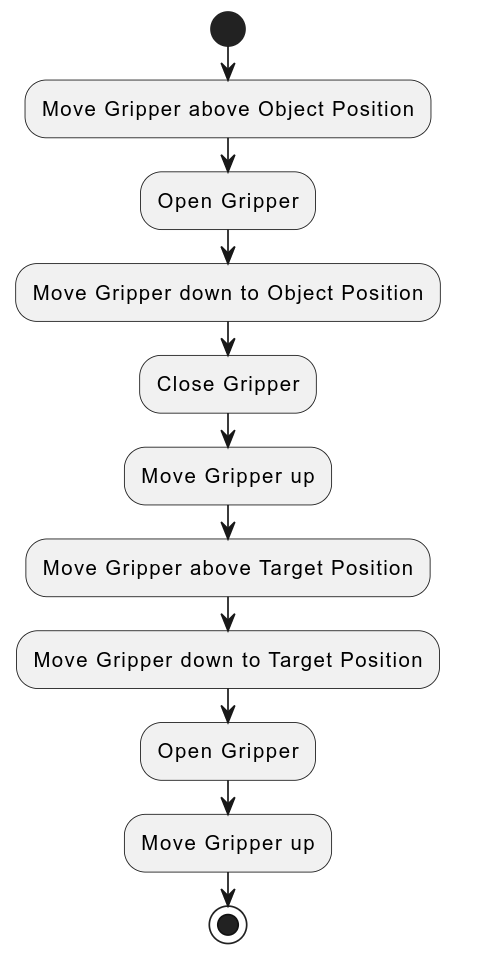
\includegraphics[width=0.5\textwidth]{Figures/pick_place_loop.png}
    \caption{Pick and place implementation}
    \label{fig:pick_n_place}
\end{figure}


% !TEX root = ../main.tex

\chapter{Results} % Main chapter title
    %The first task of 
\label{results} % \ref{CHX}



This chapter provides an overview of the results achieved during the development of the project. The objective of the project was to develop an autonomous system that can detect objects in a specific environment and relocate them to a designated location. In order to achieve this, a robot arm was programmed to perform a series of tasks. 

The first task was to detect the objects present in the environment using computer vision algorithms. This involved using a camera mounted on the robot arm to capture images of the workspace and then processing these images to identify the objects present. Once the objects were detected, the robot arm used its gripper to pick up each object and relocate it to a designated location. The gripper features force feedback to prevent object damage and avoid simulation glitches.


\begin{figure}[!h]
    \centering
    \adjincludegraphics[width=\textwidth]{Figures/workspace-cluttered.jpg}
    \caption{Cluttered workspace at the start of the simulation }
    \label{fig:workspace_start}
\end{figure}

\Vref{fig:workspace_start} shows the starting configuration of the simulation. The objects are randomly positioned on the table and the robot controller prepares the task by moving the arm into starting position and calling the object detection routine.

\begin{figure}[!h]
    \centering
    \adjincludegraphics[width=\textwidth]{Figures/workplace-organized.jpg}
    \caption{Organized workspace at the end of the routine }
    \label{fig:workspace_end}
\end{figure}

\Vref{fig:workspace_end} presents the organized workspace at the end of the simulation. The robot arm has successfully detected and relocated all objects to their designated locations within the workspace.

Ultimately, it can be concluded that the objectives and requirements of the project have been fulfilled. It's important to note that the results presented in the project report were obtained in a simulation environment, which offers certain advantages and limitations. While the simulation allowed for a controlled and repeatable setup, it didn't include the nuanced challenges of real-world applications. For instance, in the simulation, all objects were of the same size, and only one type of object was present in each class. In real-world scenarios, objects may come in different shapes, sizes, and colors. Nevertheless, the simulation provided a proof of concept for the project, which can be further refined and adapted to more complex scenarios.

\chapter{Conclusions} % Main chapter title

\label{conclusions} % \ref{CHX}


In this project a robot controller for a robot arm that can be used to organize a workspace was successfully developed. The milestones achieved in the development process included the successful implementation of computer vision techniques, the creation of a framework to automate the process of creating training data and robot arm as well as gripper movement routines.

The framework created to automate the process of training data generation is transferable to other projects in webots and possibly real world applications, depending on the quality of the object models, including their polygon density and texture resolution. Further projects could incorporate this approach and utilize a more realistic object animation to train a model for a real world use case. 

The robot controller as implemented in this project has the potential of being used in real world applications due to its simplicity and deterministic nature, increased safety due to the predictability of its movements and the ability of the inverse kinematics implementation to allow for a deterministic computation time in time critical scenarios.

Despite the project successfully achieving its objectives, there is still room for improvement. The framework implemented to automate the process of training data generation should include more configurations to set up the environment. This includes the ability to utilize different objects of the same class, as well as the ability to use multiple objects of the same class in the same scene. Improving the training data, by adding further configurations to the framework, and the training process to prevent overfitting, are key areas for future development.

One aspect of the robot's movement implementation that could be considered a significant limitation in some applications is the inability to grab and position objects from different orientations. If for example the robot arm was to be used to pick up objects from a shelf, it would be necessary to be able to grab objects from the front. While this adaptation could be easily made, having to consider objects in a shelf and a table might prove to be more challenging. 
Another aspect that could be improved is the movement of the gripper's fingers, which has its fingertips moving in a bow shape when being opened or closed. This leads to them not being able to grasp thin flat objects from the surface, like a ruler or a knife for example. This could be improved by making use of the second joint of the fingers in order to compensate for the displacement of the fingertips in the \(z\) axis.


\chapter{References for \LaTeX} % Main chapter title
\section{Result overview}
    
contamination.  The electrode takes the form of a rod or stick, leading to this process also being known as stick welding.

gas like \(CO_2\) is used or mixed in. 

    
\begin{figure}[!h]
    \centering
    \adjincludegraphics[width=0.7\textwidth,
    trim={0 {.11\height} 0 0},
    clip]{Figures/logo-thk.jpg}
    \caption{Diagram of the GMAW Method showing the electrode, the welding torch and the area around it protecting the welding site from atmospheric contamination by the shielding gas. }
    \label{fig:gmaw_nozzle}
\end{figure}
    


List:


\begin{itemize}
    \item Cracks
    \item Cavities
    \item Solid Inclusions
    \item Lack of fusion and penetration
    \item Imperfect shape and dimension
    \item Miscellaneous imperfections
\end{itemize}



\HRule\\

    
\begin{equation}
    \mathbf{X} = \left\lbrace \mathbf{x}^t,\mathbf{r}^t \right\rbrace_{t=1}^N\
    \label{eq:dataset}
\end{equation}

\begin{conditions}
    \mathbf{X} & training set\\
    \mathbf{x}^t & input variables for sample \(t\) \\
    \mathbf{r}^t & output (result) for sample \(t\) \\
    t & sample number\\
\end{conditions}

        The main hyperparameters are the following:
        \begin{description}
            \item[\textit{Max. tree depth}] The largest amount of consecutive decision nodes in a branch before creating a leaf node.
            \item[\textit{Min. samples for each split}] The minimal amount of samples from the training set that need to reach a node before producing a split into separate branches.
            \item[\textit{Min. samples for each leaf}] The minimal amount of samples from the training set that need to reach each leaf node following a split by a decision node.
        \end{description}
        

    
        \begin{figure}[!h]
            \centering
    
            \adjincludegraphics[width=0.7\textwidth,
                            trim={{.2\width} {.11\height} 0 0},
                            clip]{Figures/logo-thk.jpg}
            \caption{Nozzle offset specified in SEP 1220 }
            \label{fig:nozzle_position}
        \end{figure}
    
    
        \begin{table}
            \begin{tabular}{l|l}
                    \showrowcolors
                    % \hline
                    Type of shielding gas & M21 (18 \% \(CO_2\))\\
                    % \hline
                    Shielding gas rate \(V_G\) & 12 l/min\\
                    % \hline
                    Welding filler material, \(d _D = 1,0 mm \) &  \makecell[tp{0.5\textwidth}]{
                        G42 3 M G3Si1 (\(R_m \leq 500 MPa\))\\
                        G46 4 M G4Si1 (\(R_m > 500 MPa\))
                    }\\
                %    \hline
                    Stick-out [mm] &    10x Wire diameter\\
                    % \hline
                    Welding speed \(v_s\) & 0,5 m/min\\
                    % \bottomrule
                    \hiderowcolors
            \end{tabular}
            \caption{Welding Parameters according to  SEP-1220. }
            \label{tab:guideline_parameters_table}
        \end{table}
    
    
    
        
        
    
        

    
\begin{figure}[!h]
    \begin{subfigure}[b]{\textwidth}
        
\includegraphics[width=\textwidth]{Figures/logo-thk.jpg}
        \caption{Processed radiographic image with colored ROI and pores.}
    \end{subfigure}\\
    \begin{subfigure}[b]{\textwidth}
        
\includegraphics[width=\textwidth]{Figures/logo-thk.jpg}
        \caption{Extracted ROI and detected pores through separation of the color channels of the processed radiographic image.}
    \end{subfigure}
    \caption{Extraction of porosity information from analyzed radiographic image.}
    \label{fig:pore_extraction}
\end{figure}



    This allows the arc ignition times to be detected through the intersections between the voltage signal \(V(t)\) and its Gaussian filtered form \(V_f(t)\) with a positive slope, as well as the short-circuit start at the intersections with a negative slope. (\Vref{eq:dataset})% forming the arc\_start and shortc\_start sets respectively

    \begin{align}
        V_f(t)&=G(V(t))\label{eq:v_gauss_filter}\\
        V_{diff}(t)&=V(t)-V_f(t)\label{eq:v_diff}\\
        V_{diff}(t_i)&=0 \land
        \begin{cases}
            \frac{dV_{diff}}{dt}(t_i)> 0 \; \rightarrow \text{\(t_i=\) point at arc ignition} \\
            \frac{dV_{diff}}{dt}(t_i)< 0 \; \rightarrow \text{\(t_i=\) point at short-circuit start}
        \end{cases}
        \label{eq:voltage_phase_identification}
    \end{align}

applicators' experience and the known limited repeatability of the weld porosity during the welding process. These were defined as follows:
\[Upper limit = 1.4x + 2\]
\[Lower limit = 0.6x - 0.5\]
\begin{conditions}
    \mathbf{x} & Measured porosity in percent\\
\end{conditions}
With the identified set of Hyperparameters, a new Random Forest regression model was trained on the complete dataset used during the previous procedure.


effective sample size.

\begin{figure}[!h]
    \centering
    \begin{subfigure}[b]{0.5\textwidth}
        \adjincludegraphics[width=\textwidth,
        trim={0 {0.68\height} {0.08\width} {0.1\height}},
        clip]{Figures/logo-thk.jpg}   
        \caption{Section duration = \(2s\) \\ 68.36\% within tolerances (n=1558). }
    \end{subfigure}\hfill
    \begin{subfigure}[b]{0.5\textwidth}
        \adjincludegraphics[width=\textwidth,
        trim={0 {0.68\height} {0.08\width} {0.1\height}},
        clip]{Figures/logo-thk.jpg}        
        \caption{Section duration = \(10s\) \\ 82.81\% within tolerances (n=1286). }
    \end{subfigure}\\\vspace{0.5cm}
    
    \begin{subfigure}[b]{0.5\textwidth}
        \adjincludegraphics[width=\textwidth,
        trim={0 {0.68\height} {0.08\width} {0.1\height}},
        clip]{Figures/logo-thk.jpg}        
        \caption{Section duration = \(20s\) \\ 89.75\% within tolerances (n=946). }
    \end{subfigure}

    \caption{Weld section porosity prediction - Performance evaluation using weld sections of different lengths. }
    \label{fig:rfr_evaluation_sections_diff_lengths}
\end{figure}


% \include{Chapters/Chap1}
% \include{Chapters/Chap2} 
% \include{Chapters/Chap3}

%----------------------------------------------------------------------------------------
%	THESIS CONTENT - APPENDICES
%----------------------------------------------------------------------------------------

\appendix % Cue to tell LaTeX that the following "chapters" are Appendices

% % Appendix A

\chapter{Appendix A} % Main appendix title

\label{AppendixA} % For referencing this appendix elsewhere, use \ref{AppendixA}

\iffalse
    \section{How do I change the colors of links?}
    
    The color of links can be changed to your liking using:
    
    {\small\verb!\hypersetup{urlcolor=red}!}, or
    
    {\small\verb!\hypersetup{citecolor=green}!}, or
    
    {\small\verb!\hypersetup{allcolor=blue}!}.
    
    \noindent If you want to completely hide the links, you can use:
    
    {\small\verb!\hypersetup{allcolors=.}!}, or even better: 
    
    {\small\verb!\hypersetup{hidelinks}!}.
    
    \noindent If you want to have obvious links in the PDF but not the printed text, use:
    
    {\small\verb!\hypersetup{colorlinks=false}!}.
\fi


\iffalse
\section{Table of weekly activities}
    %\begin{tabular}[c]{c|p{4cm}|p{3.3cm}}
    %    \showrowcolors
    %    Art der Tätigkeit & Abteilung & von/bis\\ \hline
    %    Praktikant & P BU Engine \& Drivetrain Systems & \ptimeperiod\\
    %    \hiderowcolors
    %\end{tabular}
%\begin{table}[ht]
%    \centering
      \begin{longtable}{c|p{13cm}}
        \showrowcolors
             \expandableinput Lists/weekly_tasks.txt
        \hiderowcolors
        \caption[Weekly Tasks]{Weekly Tasks}
        \label{tab:Tasks_Table}
    \end{longtable}
%\end{table}
\fi

%\include{Appendices/AppendixB}
%\include{Appendices/AppendixC}

%----------------------------------------------------------------------------------------
%	BIBLIOGRAPHY
%----------------------------------------------------------------------------------------

\printbibliography[heading=bibintoc]

%----------------------------------------------------------------------------------------


\cleardoublepage %Double Space needed for first pages to be printed one-sided only. 
%\clearpage



\end{document}  
